%=======================================================================
\chapter{Einleitung}
\label{sec:Einleitung}
%=======================================================================
"`In einem Praktikum erhält der Studierende die Gelegenheit, theoretisches Wissen aus dem Studium unter realen Bedingungen auf den Prüfstand zu bringen.
Die hier gemachten Erfahrungen werden in einem Praktikumsbericht zusammengefasst.
Auch wenn ein Praktikumsbericht im eigentlichen Sinne keine wissenschaftliche Arbeit darstellt, können dennoch die gleichen Anforderungen an Form und Bearbeitung gelten.
[...] Der Aufbau eines Praktikumsberichtes kann dem einer wissenschaftlichen Arbeit entsprechen, wenn er auch nicht als solche zu werten ist.
Die Verwendung von Deckblatt und Inhaltsverzeichnis vor dem eigentlichen Textteil ist auch bei dieser Art von Arbeiten sinnvoll"' (\cite{Balz2008}, S. 157 f.).

Das Deckblatt einer wissenschaftlichen Arbeit ist der erste Eindruck, der visuell wahrgenommen wird und sollte daher ansprechend und übersichtlich gestaltet sein.
Es sollte schlicht und sachlich gehalten werden ohne flächenfüllende Grafiken und Abbildungen zu verwenden (vgl. \cite{Balz2008}, S. 186).
Es ist gemeinhin üblich das Logo der Hochschule oder Fakultät auf dem Deckblatt abzubilden, allerdings wird dringend drauf hingewiesen, dass das Logo der HSHL ohne Freigabe nicht auf dem Deckblatt verwendet werden darf.
Das Deckblatt muss laut \cite[S.\,187]{Balz2008}  folgende Elemente enthalten:
\begin{itemize}
\item Name der Hochschule
\item Bezeichnung des Studiengangs
\item Anzahl der Fachsemester
\item Titel und Untertitel der Arbeit
\item Name des Autors
\item Name des Betreuers
\item Ort und Datum der Abgabe 
\end{itemize}
Konsultieren Sie die Rahmenprüfungsordnung Ihre Studiengangs für ggf. abweichende Forderungen.

Inhaltlich wird in der Einleitung die Aufgabenstellung und die Motivation der behandelten Thematik dargestellt.
Es sollen folgende Fragen beantwortet werden:
\begin{itemize}
\item Warum ist das Thema wichtig?
\item Was sind die wesentlichen Inhalte?
\item Welche Fragen will der Bericht beantworten?
\item Wie gehe ich beim Bearbeiten und Beantworten der Frage(n) vor?
\item Für welchen Zweck sollen die Ergebnisse verwendet werden?
\item Welcher technische Fortschritt ergibt sich durch die Ergebnisse? \cite[S.~27]{Karm2011}
\end{itemize}

%=======================================================================
\section{Motivation}
%=======================================================================
\subsection*{11 Gründe warum Sie \LaTeX verwenden sollten.}

\begin{enumerate}
\bfseries
\item \LaTeX\ produziert portable und konsistente Dokumente. \\ \mdseries
    Mit LaTeX  können Sie PS- und PDF-Dateien produzieren. Wenn Sie diese Dateien versenden, brauchen Sie sich keine Sorgen zu machen, dass die Person am empfangenden Ende diese nicht öffnen kann. 
    Um PDF-Dateien zu lesen, benötigt der Empfänger lediglich einen PDF-Reader wie Adobe, Sumatra, Foxit oder Evince. Diese Programme sind Freeware. Mit dem PDF-Format können Sie auch sicherstellen, dass der Empfänger exakt die Formatierung sieht, welche Sie erstellt haben. Beim Austausch von .docx-Dateien kommt es hier häufig zu Problemen, da zwei Nutzer unterschiedliche Software verwenden. Schreiben Sie beispielsweise ein Dokument mit  KWrite und sehen Sie sich das Durcheinander in OpenOffice an. Hinzu kommt, dass als Abgabeformat in Hochschulen häufig das PDF-Format verlangt wird.
\textbf{    \item \LaTeX\ bietet Ihnen alle Vorteile digitaler Formate.}\\
    Ich benutze fast ausschließlich \verb|pdflatex|, um Dokumente zu erzeugen. Das sind bei mir vorrangig Aufgabenzettel und Praktikumsleitfäden. Da die Endergebnisse PDF-Dateien sind, kann ich diese einfach archivieren. So finde ich leicht zu jedem Jahrgang die zugehörigen Aufgaben wieder. Ich arbeite so auch nahezu papierlos und archiviere alles sortiert in Ordnern in SVN oder Sciebo. So kann man auch schnell ein Dokument mit anderen teilen oder als E-Mail versenden.  Text-Dateien und .docx-Dateien sind auch gut, aber LaTeX noch hat einen für mich entscheidenden Vorteil. Dieser bildet den nächsten Punkt.
\textbf{    \item \LaTeX\ bietet hervorragende Mathematik- und Symbolunterstützung.}\\
    Als Studentin oder Student hat man oftmals mit esoterischen mathematischen und logischen Symbolen, griechischen Buchstaben, und Gott weiß was zu tun. \LaTeX\ hat eine erstaunliche Unterstützung hierfür. Wenn Sie beispielsweise eine Herleitung einer Reihenentwicklung, wie der dargestellten Taylorreihe, machen müssen, wollen Sie Ihre Zeit nicht damit verschwenden die Formeln zu setzen.
	\[\sum\limits_{n = 0}^{\inf}\frac {f^{(n)}(a)}{n!}(X - a)^{n}
\]
\LaTeX\ ermöglicht Ihnen die Formel zu "`schreiben"' und zu kopieren, so dass Sie in der kopierten Formel schnell Umformungen einfügen können.

Es ist viel einfacher die Formel in dieser Form einzugeben:    
\begin{lstlisting}
    \sum\limits_{n = 0}^{\inf}\frac {f^{(n)}(a)}{n!}(X - a)^{n}.
\end{lstlisting} 
Auf diese Weise braucht man selbst beim erstellen von komplexen Formeln die Hände nicht von der Tastatur zu nehmen.
\textbf{\item LaTeX bietet präzise Kontrolle über das Layout des Dokuments.}\\
    Ränder, Zeilenabstand, Abstände zwischen Absätzen, Sie können alle Parameter in \LaTeX\ anpassen. Sie brauchen jedoch nicht mit der Maus Lineale und Tabulatoren hin und her zuschieben, sondern können diese Layoutvorgaben zu Beginn des Dokumentes in die \LaTeX-Datei schreiben. \LaTeX\ gibt Ihnen die Möglichkeit, das Layout bis hin zur Anzahl der Pixel zwischen Kuller und den Inhalt von Aufzählungen zu steuern. Dies ist vergleichbar mit CSS und HTML und basiert auf der Grundidee der Trennung von Inhalt und Layout. Dies wird Ihnen erleichtern sich auf den Inhalt Ihrer wissenschaftlichen Arbeit zu konzentrieren, ohne dass Sie durch Layout-Aufgaben immer wieder abgelenkt werden.
\textbf{\item Sie können Makros in LaTeX verwenden.}\\
    Nun, ich bin sicher, Sie haben aus den Informatik-Vorlesungen eine wichtigen Grundsatz mitgenommen: "`Wiederholungen sind böse und sollten durch Funktionen, Schleifen oder Makros ersetzt werden."'  Verwenden von Makros spart Ihnen Arbeit und erleichtert die Wiederverwendbarkeit bei gleichzeitig Minimierung von Fehlern. \LaTeX\ ermöglicht die Verwendung von Makros in Ihrem Dokumenten. Dieses ist definitiv eine großartige Erweiterung. Das folgende Beispiel zeigt ein solches Makro, dem ein Argument (im Beispiel der Name "`Peter"') übergeben wird:

\begin{lstlisting}
    \newcommand {\helloworld} [1] {
    % Dies ist ein Makro dem ein Argument übergeben wird
    Hallo Welt an {#1}!
    }
    
    % Das Makro wird so aufgerufen
    \helloworld{Peter}
    
    % ...und ergibt nach dem Compilieren
    Hallo Welt an Peter!
\end{lstlisting} 
\textbf{\item Sie können in \LaTeX-Kommentare verwenden.}\\
    Wie Sie im obigen Quelltextauszug vielleicht bemerkt haben, können Sie Kommentare in LaTeX nutzen. Ich halte dies für sehr hilfreich, da ich Kommentare und Notizen für mich oder andere Autoren in die Dokumente einfügen kann. Diese Kommentare sind im PDF-Dokument jedoch nicht sichtbar. Der Leser merkt somit nichts von den internen Notizen. 

\begin{lstlisting}   
    % OpenOME 2.1 Tutorial
		% Noch zu erledigen:
    % - Eclipse Setup-Prozess für Einsteiger
    % - Newsgroup Einbindung
    % - Build-Anleitung
    % - Links zu externen Quellen
    % - Bugfix: setPreferredSize Methode! (siehe bug report # 1211)
\end{lstlisting} 

    Wie Sie sehen können, ist es dies sehr praktisch. Ich verwende häufig Kommentare, um meine Gedanken zu ordnen oder um Textausschnitte auszukommentieren, die ich später überarbeiten und daher nicht löschen möchte.
\textbf{\item Sie können für \LaTeX-Dateien bequem eine Versionskontrolle wie z.\,B. SVN verwenden.}\\
    LaTeX-Dateien (mit der Endung .tex) sind reiner ASCII-Klartext. Docx-Dateien hingegen sind die binäre Dateien. Dies bedeutet, dass Sie die \LaTeX-Dateien mit eine Versionskontrolle einfach verwalten können. Die gängigen SVN-Operationen wie "`revision"', "`log"' "`diff"' und "`merge"' lassen sich somit auf \LaTeX-Dateien anwenden. Ich bin sicher, Sie wissen, warum Sie eine Versionskontrolle verwenden sollten, und werde Sie daher an dieser Stelle nicht mit Details langweilen. 
\textbf{\item \LaTeX\ hat hervorragende Bibliotheken.}\\
    Sie können den Funktionsumfang bequem mit \LaTeX-Pakete und Bibliotheken erweitern. Hier gibt es Vorlagen für Dokumenten, Veröffentlichungen, Notizen, Präsentationsfolien, Grafiken uvm.
\textbf{\item Es gibt eine Menge Unterstützung und Ressourcen für Leute, die LaTeX lernen wollen.}
    Neben Google gibt es auch eine kostenloses und phänomenales \href{http://de.wikibooks.org/wiki/LaTeX-Kompendium}{Lehrbuch} für Anfänger, die LaTeX erlernen möchten \cite{Kompendium2013}. Es gibt auch eine Menge von Diskussionsforen im Internet zum Thema. Hier finden Sie für jede Frage eine passende Antwort.
\textbf{\item \LaTeX\ ist innerhalb der wissenschaftlichen Gemeinschaft bekannt.}\\
    Ernsthaft, wo haben Sie von LaTeX das erste Mal gehört? Im zweiten Semester an der Hochschule/Uni, oder? LaTeX ist recht prominent in der Wissenschaft. Wenn Sie eine Karriere in der Forschung machen möchten, werden sich LaTeX-Kenntnisse auf jeden Fall auszahlen. Ihre Professor/innen und Mitarbeiter/innen sind wahrscheinlich sehr kompetent und könnte Ihnen bei Fragen oder Problemen helfen.
    \item \textbf{Last but not Least ist \LaTeX\ eine plattformunabhängige Freeware und bietet eine perfekte Buchsatzqualität.}
\end{enumerate}
    
Dieser Abschnitt lehnt sich an den Artikel "`10 Reasons Why Computer Science Students Should Learn LaTeX"' an \cite{Hajono2010}. 

%=======================================================================
\section{Aufgabenstellung}
%=======================================================================
In diesem Abschnitt sollte die Aufgabenstellung konkret beschrieben werden. Ihr Ergebnis wird am Erfüllungsgrad der Aufgaben gemessen.

Laborversuche müssen grundsätzlich so dokumentiert werden, dass sie "`reproduzierbar"' sind.
Das bedeutet, dass alle Informationen angegeben werden müssen, um die Versuche unter den exakt gleichen Bedingungen erneut durchführen zu können.
Es muss gewährleistet werden, dass andere Personen bei einer Wiederholung der Untersuchung zu den gleichen Ergebnissen kommen.
Ein hoher Grad an Reliabilität und Messgenauigkeit ist wichtig, d.\,h. dass die Messergebnisse zuverlässig und stabil sind \cite[S.~22~f.]{Balz2008}.
Aus diesem Grund muss die Aufgabenstellen präzise formuliert und die Versuchsvorbereitung, sowie der Aufbau, die Durchführung und Auswertung detailliert geschildert werden.
%=======================================================================
\section{Projektplan}
%=======================================================================
Besonders bei ingenieurwissenschaftlichen Themen wird das Vorgehen detailliert geplant. Stellen Sie Ihren Projektplan als Gantt-Chart (vgl. Bild \ref{fig:Gantt}) vor und heben Sie notwendige Planänderungen hervor. Die Arbeitspakete sollten nachverfolgbar sein, bei Gruppenarbeiten einer Ressource zugeordnet, Vorgänger sowie Nachfolger und Meilensteine aufweisen. Die Zeiteinheit ist sinnvoll zu wählen. Arbeiten Sie an einem Projekt ganztägig oder stundenweise entscheidet die Zeiteinheit.
\begin{figure}[htbp]
	\centering
		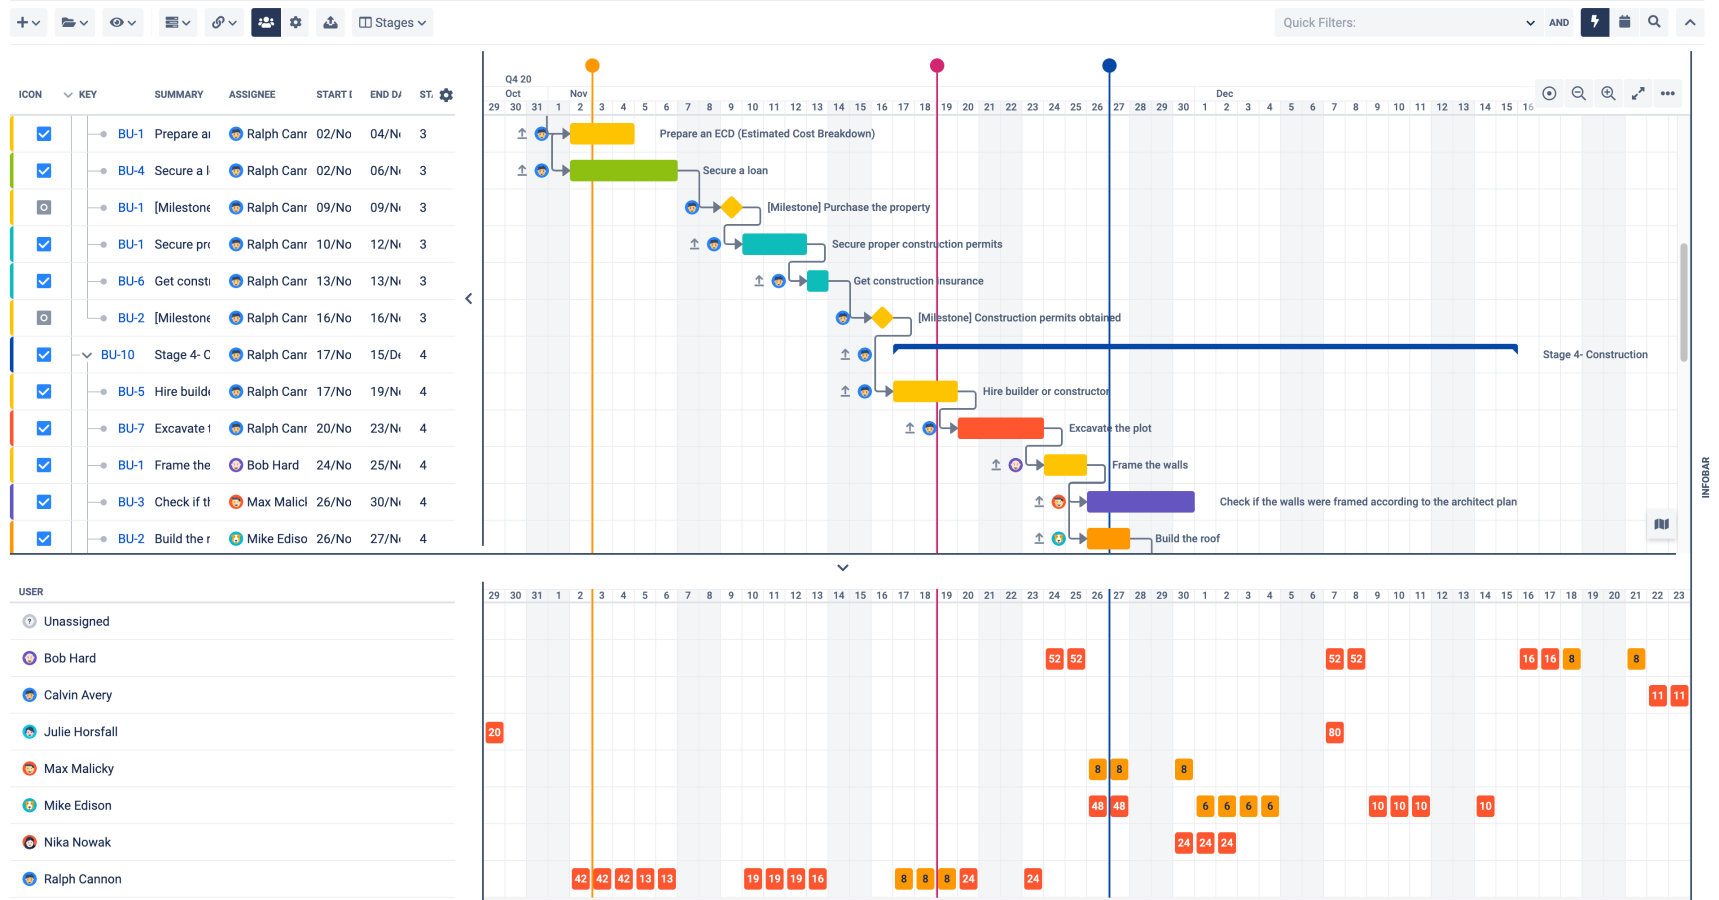
\includegraphics[width=0.90\textwidth]{Bilder/Gantt.png}
	\caption{Beispiel für ein Gantt-Chart}
	\label{fig:Gantt}
\end{figure}


%=======================================================================
\section{Gliederung}
%=======================================================================
Die Gliederung verknüpft die Aufgabenstellung mit der Lösung. Ein Beispiel könnte lauten: "`Kapitel \ref{sec:BasicRulez} beschreibt die theoretischen Grundlagen usw."'

